% Created 2017-11-17 vie 15:16
% Intended LaTeX compiler: pdflatex
\documentclass[11pt]{article}
\usepackage[utf8]{inputenc}
\usepackage[T1]{fontenc}
\usepackage{graphicx}
\usepackage{grffile}
\usepackage{longtable}
\usepackage{wrapfig}
\usepackage{rotating}
\usepackage[normalem]{ulem}
\usepackage{amsmath}
\usepackage{textcomp}
\usepackage{amssymb}
\usepackage{capt-of}
\usepackage{hyperref}
\author{Adolfo A. Bravo}
\date{\textit{<2017-05-06 sáb 10:00>}}
\title{Visualizar17}
\hypersetup{
 pdfauthor={Adolfo A. Bravo},
 pdftitle={Visualizar17},
 pdfkeywords={},
 pdfsubject={Acometer un proyecto en Medialab-Prado},
 pdfcreator={Emacs 25.2.2 (Org mode 9.1.2)}, 
 pdflang={Spanish}}
\begin{document}

\maketitle

\section*{Datalab}
\label{sec:orgf054e91}
\begin{center}

\includegraphics[width=.9\linewidth]{//logo-datalab.png}
\end{center} 

\subsection*{Actividades}
\label{sec:org69bf19b}
\begin{itemize}
\item Taller de Producción de Periodismo de Datos \emph{TPPD}
\item Taller de Visualización de Datos Visualizar \emph{V}
\item Jornadas de Periodismo de Datos \emph{JPD}
\item Día del Amor por el Software Libre \emph{ILOVEFS}
\item Día de los Datos Abiertos \emph{ODD}
\item Día de Ada Lovelace \emph{Adaday}
\end{itemize}

\section*{Medialab-Prado}
\label{sec:org2688fce}

\section*{Visualizar'17: Migraciones}
\label{sec:org74ad055}

\begin{itemize}
\item Taller Internacional de prototipado de proyectos de Visualización de Datos
\item 8 proyectos, 70 colaboradorxs
\item 10 ponentes, 12 mentorxs, 4 mediadorxs, 1 organizador, 2 apoyos.
\item 15 días: simposio, 2; taller, 12; descanso, 1; presentación: 1/2
\item Convocatoria abierta de proyectos y colaboradorxs
\item 4 entidades colaboradoras.
\end{itemize}

\subsection*{Alianzas}
\label{sec:org519870a}
\begin{center}
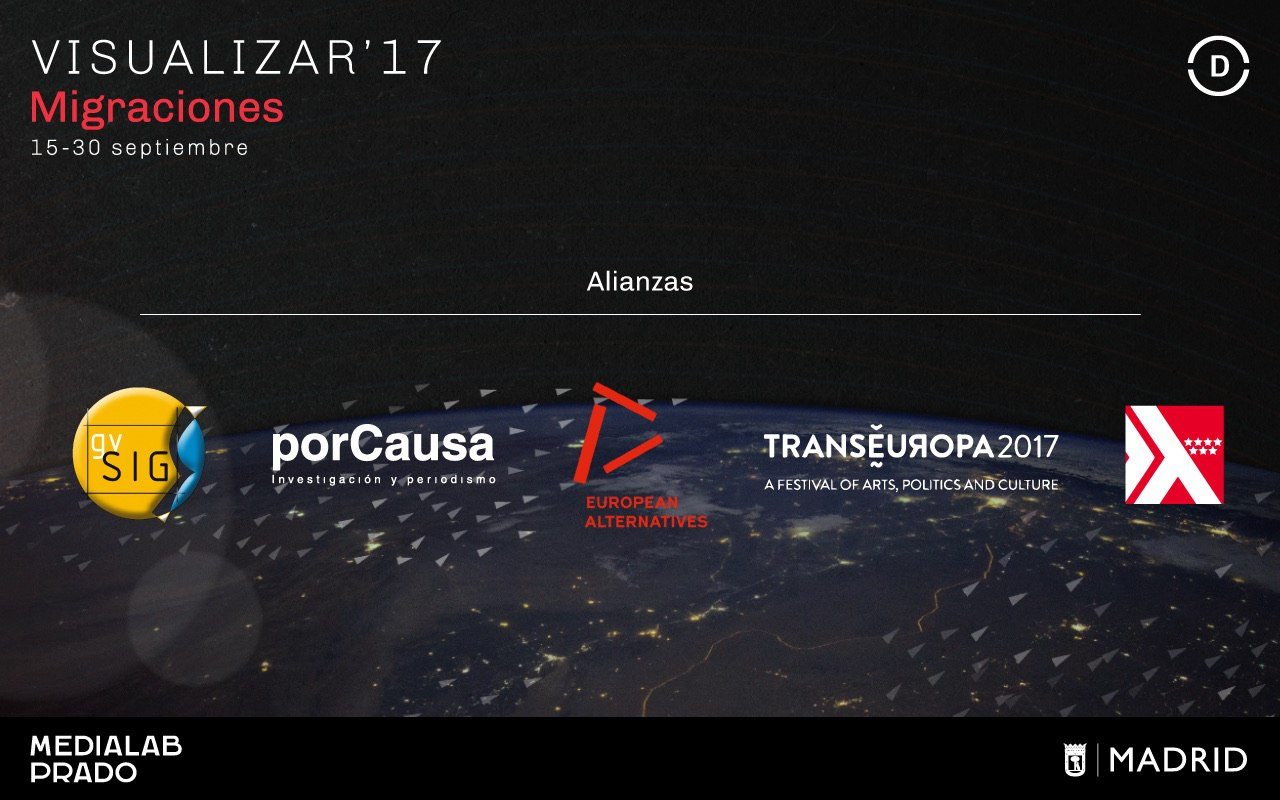
\includegraphics[width=.9\linewidth]{//alianzas.png}
\end{center}

\begin{itemize}
\item PorCausa
\item GVSIG
\item Transeuropa Festival
\item Haskell Group Madrid
\end{itemize}

\subsection*{Ponentes}
\label{sec:orgc76e96f}
\begin{center}
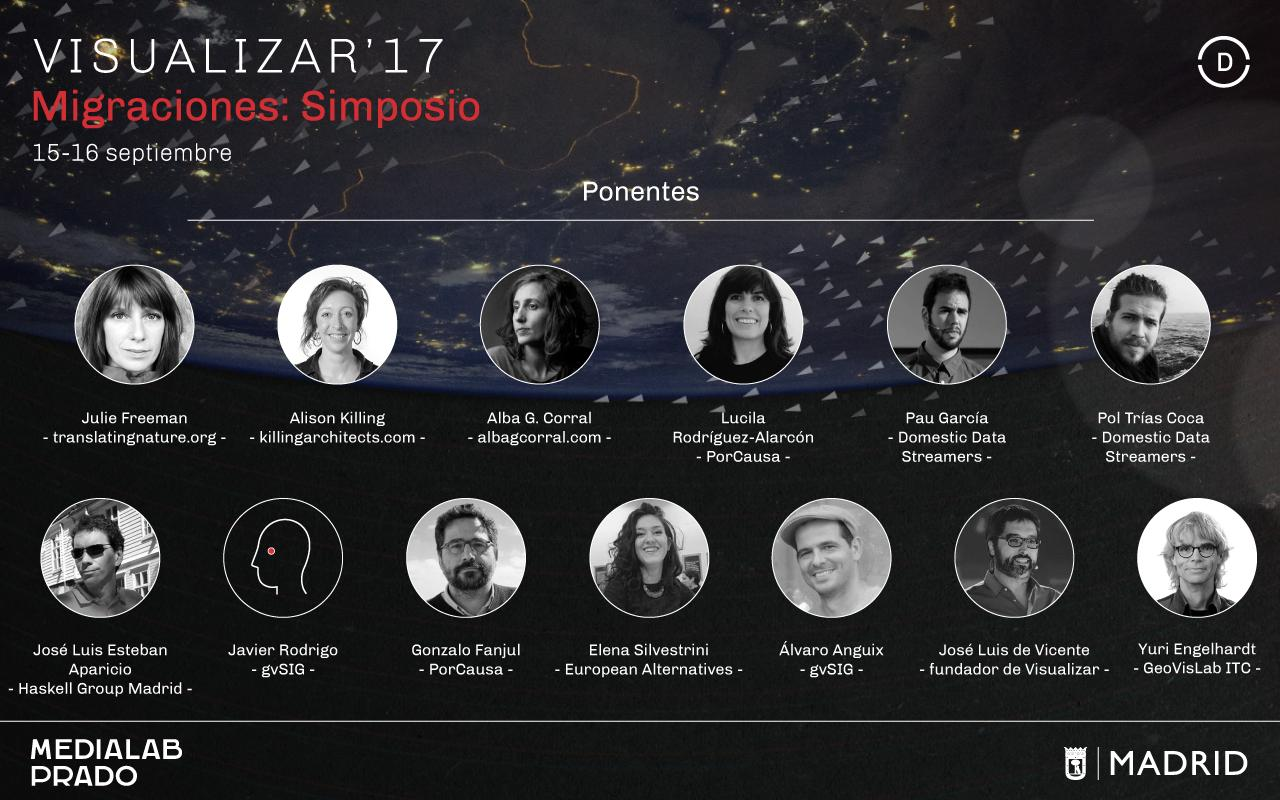
\includegraphics[width=.9\linewidth]{/ponentes-con-yuri.png}
\end{center}

\begin{itemize}
\item Alba G. Corral
\item Domestic Data Streamers
\item Alison Killing
\item Julie Freeman
\item Álvaro Anguix
\item Yuri Engelhardt
\end{itemize}

\subsection*{Comunicación}
\label{sec:orgbcee51f}


\section*{Proyectos}
\label{sec:org4fd7846}
\begin{itemize}
\item Agrega.la: \url{http://agrega.la}
\item Cerebros en movimiento: \url{https://cerebrosenmovimiento.github.io/proyecto/index.html}
\item Historia de Zainab: \url{http://historiadezainab.org}
\item Mobilomics: \url{https://medialab-prado.github.io/mobilomics/}
\item Población dirigida: \url{https://cerebrosenmovimiento.github.io/}
\item Planeta excedencia
\item Soy de Temporada: soydetemporada.es
\item Trackula: \url{http://trackula.org}
\end{itemize}
\section*{Agrega.la}
\label{sec:org3658797}
\section*{Cerebros en Movimiento}
\label{sec:org2e958ef}
\begin{itemize}
\item Orcid, plataforma digital creada en 2012.
\item Facilita un identificador numérico único (ID) a cada investigador o científico que se registre gratuitamente.
\item Hay cerca de 3 millones de usuarios.
\item Importantes editores, académicos e instituciones demandan como requisito una identificación de Orcid.
\end{itemize}
\subsection*{\url{https://cerebrosenmovimiento.github.io/}}
\label{sec:org4092811}
\section*{Historia de Zainab}
\label{sec:orgbcdf5c9}

\subsection*{historiadezainab.org}
\label{sec:orge95c2ad}

\section*{Mobilomics}
\label{sec:org2cbb479}
\begin{itemize}
\item Estudia la relación entre la movilidad y la contaminación de un día cotidiano en Madrid
\item 20 septiembre 2017
\item Utiliza publicaciones geolocalizadas en Twitter e Instagram.
\item Datos de la contaminación de Madrid y del tráfico.
\item Ilustraciones.
\end{itemize}

\subsection*{medialab-prado.github.io/mobilomics/}
\label{sec:org5d9422b}

\section*{Población dirigida}
\label{sec:org31af1b0}
\begin{itemize}
\item 1939-1973, el Instituto Nacional de Colonización (INV) promovió la construcción en España de más de 300 pueblos.
\item Creación de amplias zonas de regadío y el aumento de su productividad.
\item Se movilizaron aproximadamente a 55.000 familias.
\item Movimiento migratorio de mayor envergadura promovido por el Estado español en el siglo XX.
\item La colonización fue un proceso multidimensional caracterizado por una toma abundante de datos.
\item Territorio de datos es un grupo multidisciplinar interesado en la investigación en torno al territorio y sus dinámicas.
\end{itemize}

\subsection*{territoriodatos.org/poblacion-dirigida}
\label{sec:org0224330}

\section*{Planeta excedencia}
\label{sec:orgf3f8695}
\begin{itemize}
\item Un planeta de 40.500 personas que migran en 2016 por el cuidado personas a su cargo.
\item Esta fórmula pretende conciliar la vida familiar y laboral.
\end{itemize}
. Como norma general, se asegura el puesto de trabajo el primer año.
\begin{itemize}
\item ¿Quiénes son sus habitantes?
\item ¿Se produce un retorno al mundo laboral?
\end{itemize}
\subsection*{planetaexcedencia.es}
\label{sec:org0486037}

\section*{Soy de Temporada}
\label{sec:orgc6288f0}
-Comer productos de temporada es bueno para tu salud, tu bolsillo y el medio ambiente.
\begin{itemize}
\item Reduce las emisiones de CO2
\item Apoyas la sostenibilidad de la tierra
\item Consumes productos que han sido recogidos en su punto óptimo de maduración
\item Participas de un precio justo
\item Favoreces la economía local.
\end{itemize}
\subsection*{soydetemporada.es}
\label{sec:orgadbff12}


\section*{Trackula}
\label{sec:org18ea1da}
\begin{itemize}
\item Visualización interactiva de tu rastro en internet y de qué sitios web te rastrean a través de los contenidos que visitas cada día.
\item \url{http://trackula.org}
\end{itemize}

\begin{quote}
Para explicar cómo funcionan las interconexiones en la web utilizamos como metáfora las setas, ya que el micelio de las mismas (con lo que absorben nutrientes de la tierra) está unido bajo tierra e interconecta a los hongos.

Las setas son las páginas web que visitas conscientemente al navegar, y los puntos en los que se interconectan con otros son recursos de terceros que se encuentran incrustados tanto en una como en otra web.
\end{quote}
\subsection*{trackula.org}
\label{sec:org7049415}
\end{document}
